\chapter{Camera and object GUI main controls}
\minitoc  

%\section{Open and save data }
%\section{Undo and redo actions }

 \section{Camera controls}
Most camera related controls lay on the left part of the main window.
\subsection{Camera rotation center}
By default, the camera rotates around the origin of the coordinate system (x=0, y=0, z=0), but by pressing ``
\includegraphics[scale=0.7]{images/06/camera/move_cam.png}"/``\includegraphics[scale=0.7]{images/06/camera/move_cam2.png}", the camera will revolve around the center of mass of all opened objects. The latter option is useful when the centre of mass of an object (or of several ones) is far from the origin of the coordinate system. The grid is drawn using different colors depending on the camera rotation centre (see Fig. \ref{grid_color}). %The camera centre can also be set at the location of one of the first 10 ``normal" landmarks (see section \ref{camera_centre_at}).

\begin{figure}
  \centering
  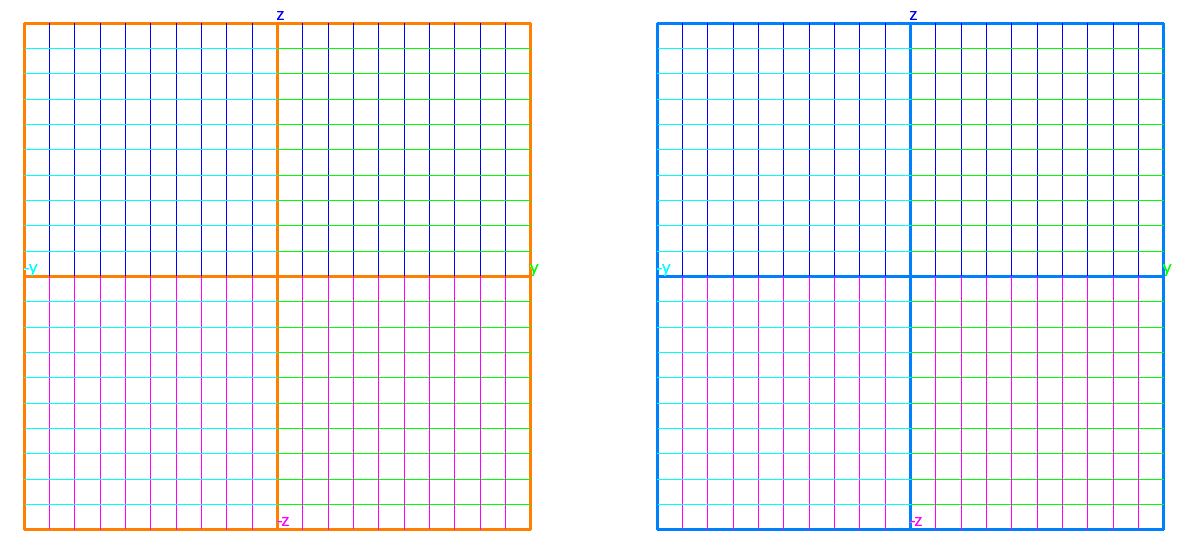
\includegraphics[scale=0.4]{images/06/camera/grids.png} 
	\caption{Grid display color. Left: when the camera revolves around the origin of the coordinate system (x=0, y=0, z=0), the grid outline is displayed in orange. Right: when the camera revolves around the center of mass of all opened objects, the grid has a blue outline.}
\label{grid_color}
 
\end{figure}

 
\subsection{Orthographic or perspective projection}
You can switch between orthographic and perspective projection mode by pressing the "
\includegraphics[scale=0.7]{images/06/camera/camera_ortho.png}" or "
\includegraphics[scale=0.7]{images/06/camera/camera_persp}" toggle button.
Note that in orthographic projection mode 
\includegraphics[scale=0.7]{images/06/camera/camera_ortho.png}, some display information regarding the grid and pixel size appear on the right bottom corner of the screen: 
\includegraphics[scale=0.7]{images/06/camera/grid_infos.png}. 


\subsection{Camera orientation}
6 camera positions are predefined :\\

\includegraphics[scale=0.7]{images/06/camera/camera_right.png} view object from right side \\

\includegraphics[scale=0.7]{images/06/camera/camera_left.png} view object from left side\\

\includegraphics[scale=0.7]{images/06/camera/camera_front.png} view object from front side (default camera position)\\

\includegraphics[scale=0.7]{images/06/camera/camera_back.png} view object from back side\\

\includegraphics[scale=0.7]{images/06/camera/camera_above.png} view object from above\\

\includegraphics[scale=0.7]{images/06/camera/camera_below.png} view object from below\\

\subsection{Camera rotation around ``z" viewing axis}

\begin{minipage}{0.7\textwidth}
To do so, you may use the slider lying around the center of the left panel of the main window.
\end{minipage}    
\begin{minipage}{0.25\textwidth}\centering
  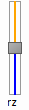
\includegraphics[scale=0.7]{images/06/camera/rz_cam.png}
 \captionof{figure}{Camera ``z" rotation slider}
 \end{minipage}    



\subsection{Clipping plane}

\begin{minipage}{0.7\textwidth}
In some cases, you may need to displace the viewing clipping plane. To do so, use
the slider lying centrally in the left panel of the main window.\\
%You can also modify the clipping plane manually by editing the ``Tz" control in the camera options window (viewing opt. $\rightarrow$ Camera $\rightarrow$ Camera options).

The button 
\includegraphics[scale=0.7]{images/06/camera/cpon.png} or 
\includegraphics[scale=0.7]{images/06/camera/cpoff.png}  permits to adjust / readjust the position of the clipping plane at predefined positions :
\begin{itemize}
\item  
\includegraphics[scale=0.7]{images/06/camera/cpon.png}: the clipping plane is placed at z = 0 (all objects having a z coordinate along
z viewing axis smaller than 0 are hidden).
\item	
\includegraphics[scale=0.7]{images/06/camera/cpoff.png} : the clipping plane is replaced at its original value : z= - camera.far / 2. This value permits to
view objects having positive and negative coordinates along z viewing axis.

\end{itemize}
\end{minipage}    
\begin{minipage}{0.25\textwidth}\centering
  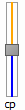
\includegraphics[scale=0.5]{images/06/camera/cp_slider.png}
 \captionof{figure}{Camera clipping plane slider}
 \end{minipage}   




\subsection{Zoom}
There are three main ways to modify the ``zoom" in MorphoDig :


\begin{minipage}{0.7\textwidth}
\begin{itemize}
\item You may use the zoom slider laying in the lower part of the left panel of the main window.
\item	You may set manually the display scale (Edit $\rightarrow$  Edit size unit and grid spacing, then define the display scale: 100 pixels in size unit). This option is only available in orthographic projection mode 
\includegraphics[scale=0.7]{images/06/camera/camera_ortho.png}.
\item	You may use the middle click mouse roll button (roll the wheel).
\end{itemize}
\end{minipage}    
\begin{minipage}{0.25\textwidth}\centering
  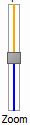
\includegraphics[scale=0.7]{images/06/camera/zoom_slider.png}
 \captionof{figure}{Zoom slider}


 \end{minipage}    




\section{Other display controls}



\subsection{Grid}
Press 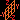
\includegraphics[scale=0.7]{images/06/other/grid.png} to show / hide the grid. Default grid size is 1 cm / square. Grid size can be edited manually
(viewing opt. $\rightarrow$ Grid size).
Switching between the 6 camera predefined positions defined above (
\includegraphics[scale=0.7]{images/06/camera/camera_right.png}, 

\includegraphics[scale=0.7]{images/06/camera/camera_left.png}, 

\includegraphics[scale=0.7]{images/06/camera/camera_front.png}, 

\includegraphics[scale=0.7]{images/06/camera/camera_back.png}, 

\includegraphics[scale=0.7]{images/06/camera/camera_above.png} and 

\includegraphics[scale=0.7]{images/06/camera/camera_below.png})
will affect the plane in which the grid is drawn.




\subsection{Coordinate system orientation helper}
\begin{minipage}{0.7\textwidth}
Press 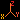
\includegraphics[scale=0.7]{images/06/other/orientation_helper.png} to show / hide the coordinate system orientation helper lying on the bottom left corner of the main 3D window. By default, the labels are defined
the following way:\\
+z axis : dorsal side\\
-z axis : ventral side\\
+y axis : left side\\
-y axis : right side\\
+x axis : anterior side\\
-x axis : posterior side.\\
You may edit these labels depending on your preferences (for instance,
depending on the structure you are working with, you may need to set ``+y" to ``labial", and ``-y" to
``lateral"). To edit orientation labels, click on ``Edit $\rightarrow$ Edit orientation labels."
\end{minipage}    
\begin{minipage}{0.3\textwidth}\centering
 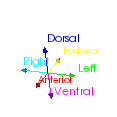
\includegraphics[scale=0.7]{images/06/camera/orientation_helper_view.png}
 \captionof{figure}{Orientation helper}
 \end{minipage}   


\subsection{Anaglyph}
Press 
\includegraphics[scale=0.7]{images/06/other/anaglyph.png} to activate/deactivate anaglyph 3D rendering.

\subsection{Lightning}
6 lightning orientations are predefined :\\

\includegraphics[scale=0.7]{images/06/other/light_right.png}light from right viewing side\\

\includegraphics[scale=0.7]{images/06/other/light_left.png}light from left viewing side\\

\includegraphics[scale=0.7]{images/06/other/light_front.png}light from front viewing side\\

\includegraphics[scale=0.7]{images/06/other/light_back.png}light from back viewing side\\

\includegraphics[scale=0.7]{images/06/other/light_above.png}light from above\\

\includegraphics[scale=0.7]{images/06/other/light_below.png}light from below\\

  \section{Object controls}
	As seen earlier, selected objects can be translated and rotated using the mouse left and middle buttons
(in landmark and camera selection modes, you also need to maintain ``CTRL" button pressed
while dragging the mouse to achieve rotation and translation of selected objects). Alternatively, you
may also use the following controls to accomplish rotation and translation of selected objects. Rotation
is performed around the global center of mass of all selected objects.

\subsection{Rotation around and translation along ``z" viewing axis}

\begin{minipage}{0.7\textwidth}
These controls are extremely useful, as there is no way to achieve rotation
around « z » viewing axis or translation along ``z" viewing axis using the
mouse. \\
To do so, use the slider and roller lying in the upper part of the left panel of the
main window.

\end{minipage}    
\begin{minipage}{0.25\textwidth}\centering
  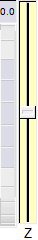
\includegraphics[scale=0.5]{images/Icons/x_rot.png}
 \captionof{figure}{Object ``z" rotation roller and slider}
 \end{minipage}    


\subsection{Rotation around ``x" and translation along ``y" viewing axes}

\begin{minipage}{0.7\textwidth}
To do so, use the slider and roller lying in the lower part of the left panel of the
main window.
\end{minipage}    
\begin{minipage}{0.25\textwidth}\centering
  \includegraphics[scale=0.5]{images/Icons/y_rot.png}
 \captionof{figure}{Object ``x" roller and ``y" slider}
 \end{minipage}   

\subsection{Rotation around ``y" and translation along ``x" viewing axes}


\begin{minipage}{0.5\textwidth}
To do so, use the slider and roller lying in the left part of the bottom panel of the
main window.
\end{minipage}    
\begin{minipage}{0.4\textwidth}\centering
  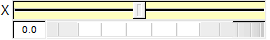
\includegraphics[scale=0.5]{images/Icons/z_rot.png}
 \captionof{figure}{Object ``y" roller and ``z" slider}
 \end{minipage}   

